\documentclass[a4paper,12pt]{book}
\usepackage[dvipdfmx]{graphicx,color,hyperref}
%\usepackage[top=30truemm,bottom=30truemm,left=30truemm,right=30truemm]{geometry}
\usepackage[a4paper,width=150mm,top=25mm,bottom=25mm]{geometry}
\usepackage{here}
%
% ハイパーリンクを付ける設定
\usepackage{pxjahyper}
\hypersetup{
  colorlinks=true,
  linkcolor=blue,
  bookmarks=true, 
  bookmarksnumbered=true,
  pdfborder={0 0 0},
  bookmarkstype=toc
}
% 本文
\begin{document}
\setcounter{tocdepth}{2}
\tableofcontents


\section{Introduction}
\subsection{KAGRA Site}
\section{Theory of Seismic Waves}
\subsection{Body Waves}
\subsection{Surface Waves}
\section{}
\section{Seismic Noise}

\section{基線長伸縮}
地面振動は共振器を同相と逆相に動かす。同相は共振器の重心移動成分で逆相は共振器長伸縮成分である。同相と逆相成分は独立しているが、共振器鏡の地面応答がITMとETMで異なると同相から逆相成分へのカップリングが生じる。このカップリングは同相雑音除去比または Common Mode Rejection Ratio (CMRR) として知られている。CMRRが大きいと同相入力は逆相へカップルしにくくなる。一方で地面振動は二点間の距離が弾性波の波長に対して十分小さければ、ほとんど同相で動き、逆相成分を持たない。本章ではこの逆相の低減比をCommon and Differential Ratio (CDMR) として定義する(式\ref{eq:eq23})。\footnote[3]{このCDMRのことをCMRRと言っている場面がみられるが、それは正しくないように思う。元来、CMRRは差動増幅器の同相入力応答と逆相入力応答の比で定義されている。これはシステムに同相で入力したときにどれだけ逆相にカップルするかというカップリング係数である。CDMRは、システムに入力される同相と逆相成分がどの程度の割合なのかという量である。}CDMRが大きければITMとETMの逆相成分は同相成分より小さくなる。以上のことから、共振器長制御にとって、「CDMRの大きい地面にCMRRの高い共振器を置くこと」が大事であるといえる。

後述するようにCDMRは、基線長と弾性波の位相速度に依存する。基線長が長く位相速度が遅くなれば2点間のコヒーレンスが悪くなり、CDMRは小さくなる。CDMRをKAGRAとVirgoで比較すると、$0.2\, \mathrm{Hz}$でおよそ10倍ほどKAGRAのほうが大きく、基線長伸縮が低減されていることがわかった。

\subsection{同相成分と逆相成分}
\begin{figure}[H]
  \begin{center}
    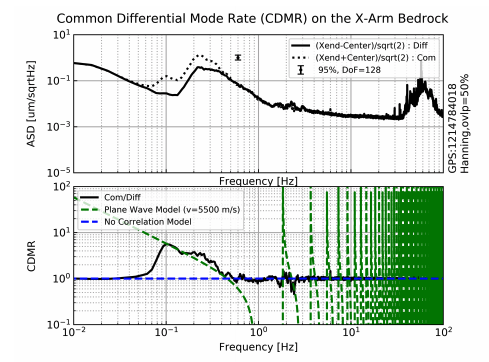
\includegraphics[width=8.0cm]{./img_cdmr_xarm.png}
  \end{center}
  \caption{2点の変位。変位場を$u(t,x)$とすれば、$x_1,\,x_2$それぞれの変位は$u(x_1,t),\,u(x_2,t)$である。}\label{img:img_diffcomm}
\end{figure}

図\ref{img:img_diffcomm}で示すような2点$x_1,\,x_2$について、変位の同相成分と逆相成分を定義する。それぞれの変位は変位場$u(x,t)$をもちいて$u(x_1,t),u(x_2,t)$となる。ここで,これら2つの変位の同相成分$u_{\mathrm{comm}}$と逆相成分$u_\mathrm{diff}$を
\begin{eqnarray}\label{eq:eq22}
  u_{\mathrm{diff}} \equiv \frac{u_{1}-u_{2}}{\sqrt{2}},
  u_{\mathrm{comm}}  \equiv \frac{u_{1}+u_{2}}{\sqrt{2}}
\end{eqnarray}
と定義する。パワーが保存するように規格化定数は$\sqrt{2}$にしている。同相成分は2点の重心移動をあらわし,逆相成分は2点の基線長伸縮を表す。


\subsection{Common and Differential Mode Ratio (CDMR)}
離れた2点がどれぐらい同相で動くか評価する指標として、同相と逆相成分の比である Differential Mode Rejection Ratio (CDMR) を以下のとおり定義する。
\begin{equation}
  \boxed{\mathrm{CDMR} \equiv \sqrt{\frac{同相成分のパワー}{逆相成分のパワー}} = \sqrt{\frac{P_{\mathrm{comm}}(\omega)}{P_{\mathrm{diff}}(\omega)}}} \label{eq:eq23}
\end{equation}

$P_{\mathrm{comm}},P_{\mathrm{diff}}$は同相成分と逆相成分についてのパワースペクトル密度である。パワースペクトル密度は自己相関関数$C(\tau)$をフーリエ変換したものなので、まず自己相関関数$C_{\mathrm{diff}}$を求める。自己相関関数$C_{\mathrm{diff}}$は,各々の自己相関を$ C_{ij} \equiv \langle x_{i}(t)x_{j}(t+\tau)\rangle,\, (i=1,2,\,j=1,2)$と定義すれば, 
\begin{eqnarray}
  C_{\mathrm{diff}}(\tau) &=& \frac{1}{2}
  \biggl\langle
  \biggl[ x_{1}(t)-x_{2}(t) \biggr] \biggl[ x_{1}(t+\tau)-x_{2}(t+\tau) \biggr]
  \biggr\rangle \\
  &=& \frac{1}{2}\biggl[ C_{11}(\tau) - C_{12}(\tau) - C_{21}(\tau) + C_{22}(\tau) \biggr], 
\end{eqnarray}
となるので、これをフーリエ変換すれば逆相成分のパワースペクトル密度$P_{\mathrm{diff}}(\omega)$は
\begin{eqnarray}
  P_{\mathrm{diff}}(\omega) &=& \frac{1}{2}\biggl[ P_{1}(\omega) + P_{2}(\omega) - P_{12}(\omega) - P_{12}^*(\omega) \biggr]\\
  &=& \frac{1}{2} \biggl[ P_{1}+P_{2} - \mathrm{Re}\left[\mathrm{coh} \right]\times2\sqrt{P_{1}P_{2}} \biggr] \label{eq:eq31}
\end{eqnarray}
となる。$P_{1}(\omega),P_{2}(\omega)$はパワースペクトル密度、$P_{12}(\omega)$はクロススペクトル密度、$\mathrm{coh}$は以下の通り定義されたコヒーレンスである。
\begin{eqnarray}
  \mathrm{coh} \equiv \frac{P_{12}}{\sqrt{P_{1}P_{2}}}
\end{eqnarray}


さてここで、2箇所でののパワースペクトル密度$P_{1},P_{2}$が同じだと仮定してCDMRを求めてみる。\footnote[3]{この仮定は、振幅が減衰しない弾性波が地面を伝搬するような場合でのみ適用できる。局所的な励起源がない場合や、脈動のような等方に励起源があるような場合で適用できるはず?}つまり$P_{1}=P_{2}\equiv P$とすることができて、$\mathrm{CDMR}$は定義式(\ref{eq:eq23})より、
\begin{eqnarray}
 \mathrm{CDMR} = \sqrt{\frac{1 + \mathrm{Re} \left[\mathrm{coh} \right] }{1 - \mathrm{Re} \left[\mathrm{coh} \right]}} \label{eq:eq33}
\end{eqnarray}
と書き表すことができる。
式(\ref{eq:eq33})からわかるように、同相成分と逆相成分のパワー比は2つの信号のコヒーレンスであらわすことができる。コヒーレンスが1の場合は2点間が同相でうごき逆相成分を持たないのでCDMRは無限大になり、一方でコヒーレンスが-1の場合は逆相成分しか持たずCDMRは0になる。またコヒーレンスが0の場合はCDMRは1になる。

なおコヒーレンスが既知で地面振動の振幅スペクトル密度が全域で同じ場合1点の地面振動から逆相成分を計算することが可能である。式(\ref{eq:eq31})をつかって、
\begin{eqnarray}
  P_\mathrm{diff} = P \sqrt{1 - \mathrm{Re[coh]}} \label{eq:eq34}
\end{eqnarray}
となる。コヒーレンスは次項で述べる弾性波モデルを仮定すれば計算することが出来るため、1点の地面振動から基線長伸縮を求める場合に便利である。


\subsubsection{単一平面波モデル}
ある方向から平面波が伝搬する場合のCDMRを求める。これは励起源が1箇所の場合に適用できる。
平面波がx軸からみて方位角$\theta$から到来するとする。つまりx軸方向では平面波の波長は$\lambda=\lambda/\mathrm{cos}\theta$になる。この場合$\tau=L\mathrm{cos}\theta/c$ほど遅れて$x_1$の変位が$x_2$へ伝達すると考えることができるので、その伝達関数はむだ遅れ要素$e^{i(L\mathrm{cos}\theta/c)\omega}$になる。2点のパワーが同じであればコヒーレンスは伝達関数と等しくなるので、コヒーレンスは
\begin{equation}
  \mathrm{coh}=e^{i\frac{L\mathrm{cos}\theta\omega}{c}}
\end{equation}
になる。CDMRは以下の通りである。
\begin{equation}  \label{eq:eq18}
  \mathrm{CDMR} = \sqrt{\frac{1+\mathrm{cos}(\frac{L\omega}{c}\mathrm{cos}\theta)}{1-\mathrm{cos}(\frac{L\omega}{c}\mathrm{cos}\theta)}}
\end{equation}



\subsubsection{等方モデル}
平面波が等方的に伝搬する場合のCDMRを求める。これは励起源が等方に存在する場合に適用できる。式(\ref{eq:eq18})をすべての方位について積分すると求まる。ただしコヒーレンスが1になるように全方位角で割って規格化する。つまりコヒーレンスの方位平均は、
\begin{eqnarray} \label{eq:eq19}
  \mathrm{coh} &=& \frac{1}{2\pi} \int_{-\pi}^{\pi} e^{i\frac{\omega}{c} L\cos \theta} d \theta \\
\end{eqnarray}
となる。したがってCDMRは以下の通りになる。
\begin{equation}  \label{eq:eq20}
  \mathrm{CDMR} = \sqrt{\frac{1+J_0(\frac{L\omega}{c})}{1-J_0(\frac{L\omega}{c})}}
\end{equation}

なお、式(\ref{eq:eq19})はSPAC係数として知られている。この係数と実測されたコヒーレンスから位相速度を求めることができる。

\subsection{SPAC法による位相速度の算出}

つかれた。
グラフ貼ったのでまた明日。

\begin{figure}[H]
 \begin{minipage}{0.5\hsize}
  \begin{center}
    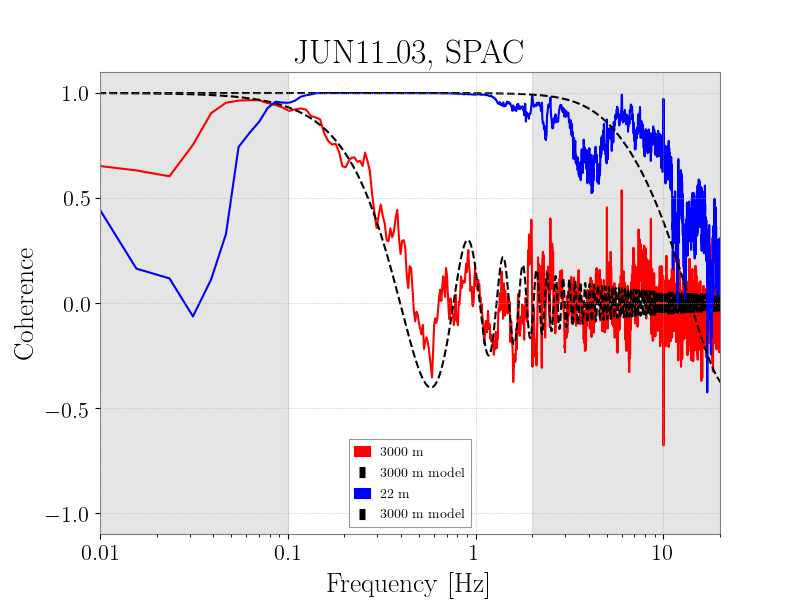
\includegraphics[width=8.0cm]{./img_coherence_result.png}    
  \end{center}
  \caption{a}
  \label{img:img_coherence_result}  
 \end{minipage}
 \begin{minipage}{0.5\hsize}
  \begin{center}
    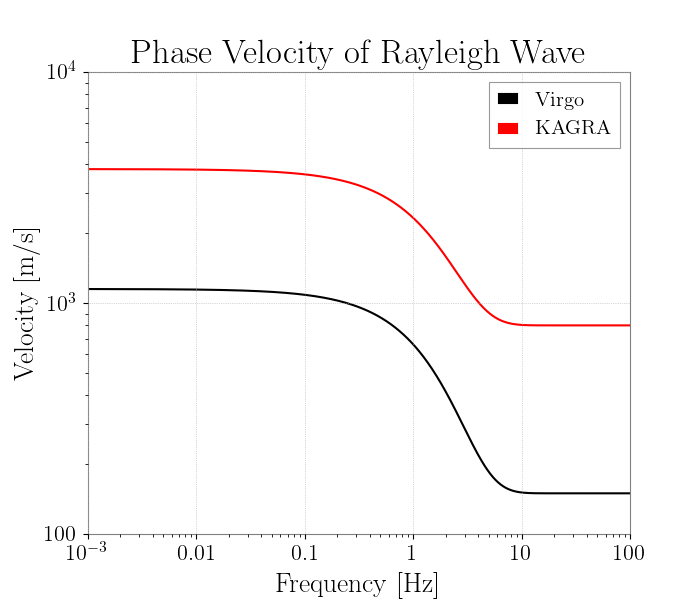
\includegraphics[width=7.0cm]{./img_RwaveVelocity.png}    
  \end{center}
  \caption{a}
  \label{img:img_RwaveVelocity}  
 \end{minipage}
\end{figure}

\begin{figure}[H]
  \begin{center}
    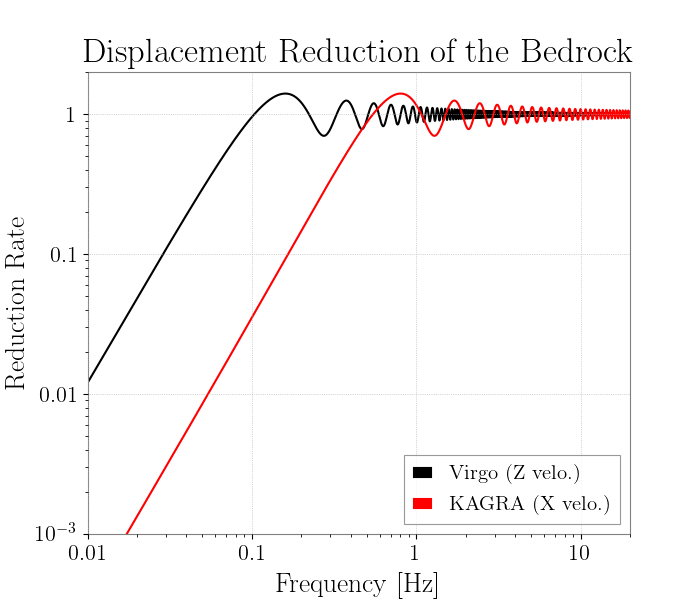
\includegraphics[width=8.0cm]{./img_CDMR.png}
  \end{center}
  \caption{}
  \label{img:img_dmrr}
\end{figure}



\appendix
%\bibliography{./reference}
\end{document}
